% -- Encoding UTF-8 without BOM
% -- XeLaTeX => PDF (BIBER)

\documentclass[espanol]{cv-style}     % Add 'print' as an option into the square bracket to remove colours from this template for printing. 
                                      % Add 'espanol' as an option into the square bracket to change the date format of the Last Updated Text
%\setdefaultlanguage{spanish}
%\sethyphenation[variant=spanish]{}{}  % Add words between the {} to avoid them to be cut 

\usepackage{graphicx}

\begin{document}

\header{Arles }{Bustamante Reyes}
\lastupdated

%----------------------------------------------------------------------------------------
% SIDEBAR SECTION  -- In the aside, each new line forces a line break
%----------------------------------------------------------------------------------------
\begin{aside}
\section{-}
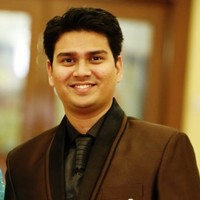
\includegraphics[width=4cm]{22}
%
\section{datos personales}
24 años, argentino
D.N.I.: 35747233
%
\section{contacto}
(011) 15 2264 1801
~
juan.alcoleas@gmail.com
~
Moreno 1836 1°A
Balvanera, CABA, Argentina
%
\section{idiomas}
Español (lengua materna),
Inglés (lectura y escritura técnicas nivel avanzado, oral nivel intermedio)
%
\section{lenguajes de programación}
{\color{red} $\varheartsuit$} Python, C, C++, Haskell, Assembler, Bash/Zsh Scripting, Java
%
\section{desarrollo web}
Flask/Tornado WEB Frameworks, Bootstrap, HTML5, CSS3, JavaScript/JNode/jQuery, Apache/Nginx WEB Servers
%
\section{tecnologías miscelaneas}
{\color{red} $\varheartsuit$} OpenSource, Gentoo/Ubuntu/Debian y otros Linux, Scrapy Crawling y Scraping Framework, NTKL (Natural Language Toolkit), RabbitMQ, MemCached, SVN/GIT Source Version Control, MySQL/PostgreSQL/ LiteSQL/MongoDB DataBases, Latex
%
\end{aside}
%----------------------------------------------------------------------------------------
% RESUMEN SECTION
%----------------------------------------------------------------------------------------
\vspace{0.2cm}
\section{Resumen}
  \vspace{-0.2cm}
Soy Analista SAP con 5 años de experiencia, en soporte y requerimientos para los diferentes módulos \textbf{SAP MM, FI, y CO. Asistencia en las casuisticas reportadas en la gestión de gastos de SAP Ariba, Ariba Network y soporte para SAP Screen Personas 2.0}.
Soy capaz de aprender de forma constante y responsable, también soy proactivo con capacidad de adaptación a los cambios, siempre busco obtener el mejor resultado posible para mi equipo.
Siempre predispuesto para resolver conflictos aportando nuevas ideas y nuevas soluciones, tengo la pasión de aventurero y querer descubrir nuevos lugares, soy capaz de captar rápidamente nuevos y diferentes procesos. 
Mis Conocimientos Fundamentos los tengo en \textbf{ITIL V3, PMBOK V5, AGILE, SCRUM, Excel Intermedio (dinamicas, VB, Cristal Reports 10, Erwin 4.0, SQL, Rational Rose 2003/2007 UML, HTML y LATEX}.
%----------------------------------------------------------------------------------------
% WORK EXPERIENCE SECTION
%----------------------------------------------------------------------------------------
\section{experiencia}
  \vspace{-0.2cm}
\begin{entrylist}
%------------------------------------------------
\entry
  {\scalebox{.8}[1.0]{2014--Actualidad}}
  {Boré Imprenta e Imagen S.A.}
  {Ciudad Autónoma de Buenos Aires, Argentina}
  {\jobtitle{Diseñador y Diagramador Senior}\\
  En la actualidad soy encargado del Departamento de Diseño y Diagramación, con personal a cargo variable (entre 1 y 3 personas) y trato fluido con los clientes. Ofrecemos soluciones para el diseño de imagen de particulares y pequeñas empresas; diagramación de catálogos, folletos y libros; así como la edición de videos para publicidad y eventos. Trabajando con tecnologías de Adobe Creative Suit (Illustrator/Photoshop/InDesign/Premier Pro/AfterEffects).}
%------------------------------------------ ------
\vspace{-0.3cm}
\entry
  {\scalebox{.8}[1.0]{2013--2014}}
  {Oony S.A.}
  {Ciudad Autónoma de Buenos Aires, Argentina}
  {\jobtitle{Desarrollador de Software Junior}\\
  Oony es una Start Up que ofrece una aplicación de Acumulación de Ofertas. Ahí adquirí una amplia batería de conocimientos en \textbf{mantenimiento de servidores} y \textbf{desarrollo de aplicaciones WEB}, tanto back-end como front-end. Específicamente la localización de errores en los servidores (control de Logs y APIs de monitoreo), su solución (desarrollo de mejoras y actualizaciones de software), el desarrollo de la aplicación WEB que concentra una gran cantidad de productos (Scalability); la obtención y el análisis del contenido (Parsing, Data Mining, Classification).\\
  \textbf{Proyectos desarrollados:}
  \begin{itemize}\small{
    \item Parseo de HTML, XML, CSV, JSON (por medio de la biblioteca Scrapy).
    \item Categorización del contenido a partir de sus descripciones\\
    (utilizando las bibliotecas NLTK).
    \item Paralelización de consultas a APIs, optimizando tiempos de respuesta\\
    (manejo de Threads).
    \item Desarrollo de APIs para back-end.}
  \end{itemize}}
%------------------------------------------------
\end{entrylist}
%----------------------------------------------------------------------------------------
% EDUCATION SECTION
%----------------------------------------------------------------------------------------
\section{educación}
  \vspace{-0.2cm}
\begin{entrylist}
%------------------------------------------------
\entry
{\scalebox{.8}[1.0]{2010--Actualidad}}
{Licenciatura en Ciencias de la Computación}
{Facultad de Cs. Exactas y Naturales, UBA}
{\textbf{Promedio: 8.8}\\
\small{Materias aprobadas y cursando: CBC aprobado con promedio 8; Álgebra 7; Análisis Matemático 9; Teoría de Juegos 10; Algoritmos y Estructuras de Datos I 10; Algoritmos y Estructuras de Datos II (Final Pendiente); Algoritmos y Estructuras de Datos III (Final Pendiente); Organización del Computador I 9; Organización del Computador II (Final Pendiente); Sistemas Operativos (Cursando); Probabilidad y Estadística (Cursando).\\
Optativas del \textbf{Departamento de Matemática}: Álgebra Lineal 8; Análisis Matemático II 9; Cálculo Avanzado (Final Pendiente)}}
%------------------------------------------------
\entry
{\scalebox{.8}[1.0]{2004--2008}}
{Bachiller \normalfont{Modalidad Ciencias Naturales}}
{EEM N° 7, 9 de Julio, Buenos Aires, Argentina}
{Promedio: 9}
%------------------------------------------------
\end{entrylist}
%----------------------------------------------------------------------------------------
% AWARDS SECTION
%----------------------------------------------------------------------------------------
\section{extracurricular}
  \vspace{-0.2cm}
\begin{entrylist}
%------------------------------------------------
\entry
{\scalebox{.8}[1.0]{2007--2008}}
{Olimpíadas Matemáticas Argentinas}
{}
{Alumno aprobado en el Certamen Nacional de las 24º y 25º Olimpíadas Matemáticas Argentinas}
%------------------------------------------------
\end{entrylist}
  \vspace{-0.2cm}
%----------------------------------------------------------------------------------------
% INTERESTS SECTION
%----------------------------------------------------------------------------------------3
\section{intereses}
  \vspace{-0.2cm}
\textbf{Back-end.} Sectores de análisis de datos y categorización (Natural Language Processing, Machine Learning); optimización de procesos; mantenimiento de servidores y bases de datos; seguridad informática.
%----------------------------------------------------------------------------------------
\end{document}
